\section{Efficient Active-Lane Consolidation}
\label{sec:approach}

This section presents an ALC design that addresses key limitations in Wyatt \etal's initial design\cite{praharenka_vectorizing_2022}. After a review of the original ALC design (\rsec{original-alc}), \rsec{gathers-scatters-are-bad} presents evidence that the higher-than-anticipated cost of the gather/scatter instructions renders Wyatt \etal's ALC ineffective.
The approach proposed in this work to eliminate gather/scatter instructions is presented in \rsec{alc-data-permutation}.
Lastly, \rsec{single-if-statement-approach} describes a novel algorithm that extracts the best of both ALC and control-flow linearization in a common case when loops have only a single \textbf{control-flow-divergent path} (\cpath).

\subsection{Original ALC Design}
\label{sec:original-alc}

Wyatt \etal propose two variations of ALC: \unrollALC and \iterALC.
In both versions, ALC is applied after \ifconversion.
In the \unrollALC, the \ifconverted and vectorized loop is unrolled once and two index vectors are formed, one for each iteration of the loop before unrolling.
Each index vector is initialized such that each lane contains the value of the loop's induction variable of each scalar iteration.

In Wyatt \etal's the path that is most likely to be taken across all iterations of the loop is chosen for consolidation based on profiling information.
Then two predicate vectors are formed by evaluating the condition to execute that path. After doing permutation, all vector operations in the consolidated path operate with uniform vectors without predication.
This work focuses on cases with small ($< 3$) paths and thus consolidation is applied to all paths.

Once the predicates are formed, the index vectors are permuted such that all active lanes are consolidated into a \emph{merged vector} \vM.
The inactive lanes are kept in a \emph{remainder vector} \vR.
Finally, if the \vM is uniform, then the consolidated uniform path is executed.
Otherwise, the \ifconverted path is executed.
The main difference between \unrollALC and \iterALC is that, in \iterALC, the \ifconverted and vectorized loop is not unrolled.
Instead, the active lanes from multiple iterations are merged into \vM until \vM is a uniform vector. 
Only then the consolidated uniform path is executed.
\iterALC works well for loops with a conditional that contains vectorizable code in both the then and the else block.
In this case, \code{then} lane are consolidated into \vM, and \code{else} lane are consolidated into \vR.
Whenever either \vM or \vR is full, the corresponding code can be executed in a uniform vector.

In both versions, any data that is dependent on the loop indices --- e.g. arrays $a$, $b$, and $c$ in \rlst{simple-loop} ---, are loaded using gather-load instructions because a consolidated vector might contain non-consecutive indices.
A gather-load instruction loads data from (potentially) non-consecutive addresses calculated by adding a base-pointer operand to each index in the index-vector operand.
Similarly, any write-back to memory needs to be performed via scatter-store instructions, which also can write into non-consecutive memory addresses.
By design, the use of gather/scatter instructions is unavoidable in Wyatt \etal's ALC.
In \rsec{gathers-scatters-are-bad}, experimental results show that gather/scatter instructions can render ALC ineffective on real hardware with SVE.

\subsection{How Gather/Scatter Instructions Hurt ALC}
\label{sec:gathers-scatters-are-bad}

\begin{center}
\begin{minipage}[t]{0.8\linewidth}
\begin{lstlisting}[
language=C,
caption={Simple conditional copy loop.},
label=lst:simple-cond-copy-loop]
for (int i = 0; i < n; i++) {
    if (cond[i]) {
        b[i] = a[i];
    }
}
\end{lstlisting} 
\end{minipage}
\end{center}


In order to understand the prohibitive overhead of gather/scatter instructions in ALC's performance, consider the simple loop in \rlst{simple-cond-copy-loop}.
The loop conditionally copies elements from array $a$ to array $b$, both are 32-bit integers.
An element $a[i]$ is copied to $b[i]$  if, and only if, the value in $cond[i]$ is true.
\rtab{gather-scatter-bad} shows performance metrics for different versions of the loop in \rlst{simple-cond-copy-loop}.
For the results in \rtab{gather-scatter-bad}, the \code{cond} array was initialized such that every other element has a \code{true} value ($50\%$ sparsity).
The results were obtained following the methodology in \rsec{methodology}.
Both \ALC and \ALCdp versions are generated by the compiler pass described in \rsec{alc-pass}.

\begin{table}[t]
\centering
\caption{Performance metrics when executing different versions of the loop in \rlst{simple-cond-copy-loop}: number of cycles to execute the loop (\textit{Total Cycles}), number of executed instructions (\textit{Num. Exec. Instructions}), cycles with no instruction completed (\textit{Stalled Cycles}), and cycles stalled due to memory operations (\textit{Memory Ops. Stalled Cycles}). Versions of the code: non-vectorized (\scalar), \ifconverted \& vectorized (\ifconv), \iterALC with gather/scatter instructions (\ALC), and \iterALC with data permutation and without gather instructions (\ALCdp).}
\label{tab:gather-scatter-bad}
\begin{tabular}{|p{1.25cm}|p{0.9cm}<{\centering}|p{1.55cm}<{\centering}|p{0.9cm}<{\centering}|p{1.85cm}<{\centering}|}
\hline
\makecell{Version\\ / Metric} &
\makecell{Loop\\ Cycles} &
\makecell{Num. Exec.\\ Instructions} &
\makecell{Stalled\\ Cycles} &
\makecell{Memory Ops.\\ Stalled Cycles} \\ \hline
\scalar &    132M &  224M &    21M &  1.6M \\ \hline
\ifconv &    14M  &   14M &     9M &  1.2M \\ \hline
\ALC    &   220M  &   16M &   210M &  110M \\ \hline
\ALCdp  &    58M  &   63M &    38M &  1.3M \\ \hline
\end{tabular}
\end{table}

Unsurprisingly, all vectorized versions of the loop --- \ifconv, \ALC, \ALC  --- execute fewer instructions than the \scalar code.
Each vector instruction in the loop operates on 16 32-bit integers at a time ($VL = 512$ bits).
However, \ALC is more than $66\%$ slower than \scalar, even while it executes $14\times$ fewer instructions, because \ALC causes $10\times$ more stalls than the \scalar code.
More than half of the stalls are due to waiting for memory stalls.
The main culprits are the gather/scatter instructions because they require multiple load/store ports instead of a single port as regular vector loads~\cite{A64FXmanual}.
In addition, in the current ARM vector-unit design, the address calculations for gather/scatter instructions are executed in the floating-point vector units~\cite{A64FXmanual}, which have higher latency than the integer operations used for regular vector loads/stores.
When Wyatt \etal evaluated their design, they had no access to hardware and thus based their evaluation on counting the number of instructions executed in a simulator.
\rtab{gather-scatter-bad} are the first results, obtained in real hardware with SVE, that show that the reduction in the number of instructions enabled by Wyatt \etal's ALC design does not translate into faster execution.
Therefore, in order for an \ALC design to have a chance at being faster than \ifconverted and vectorized code, gather/scatter instructions need to be avoided or eliminated.
\rsec{alc-data-permutation} discusses how gather instructions can be eliminated.
In \rsec{eval-scatters-costs} shows empirical results which indicate that reducing the number of scatter stores also improves ALC's performance.

\subsection{Efficient ALC via Data Permutation}
\label{sec:alc-data-permutation}

\begin{figure*}[t]
\centering
\begin{subfigure}[b]{0.325\textwidth}
\begin{lstlisting}[escapechar=|,language=PretendAsm]
vload    v1, r1 --------------->>
vload    v2, r2 --------------->>
vload    v3, r3 --------------->>
vcmp_lt  pT, v1, v2 ----------->>
vcmp_le  pF, v1, v2












vadd     v1, v1, v3, pF
vstore   v1, r1, pF




vmul     v2, v2, v3, pT
vstore   v2, r1, pT
br LATCH
\end{lstlisting}
\caption{\ifconv.}
\label{fig:simple-loop-ifconv}
\end{subfigure}%
\begin{subfigure}[b]{0.325\textwidth}
\begin{lstlisting}[escapechar=|,language=PretendAsm]
// --------------------------->>
// --------------------------->>
// --------------------------->>
// --------------------------->>




# Index vector permutation.
permute vI, vM, vR, pT, pF --->>
if_all_true vM, U_THEN ------->>
# if vM is not uniform true,
# then vR is uniform false.
swap    vM, vR --------------->>
U_ELSE:
gather  v1, r1, vM
gather  v3, r3, vM
vadd    v1, v1, v3
scatter v1, r2, vM ----------->>
br LATCH
U_THEN:
gather  v1, r1, vM
gather  v3, r3, vM
vmul    v2, v2, v3
scatter v2, r1, vM ----------->>
br LATCH
\end{lstlisting}
\caption{\ALC.}
\label{fig:simple-loop-alc}
\end{subfigure}%
\begin{subfigure}[b]{0.325\textwidth}
\begin{lstlisting}[escapechar=|,language=PretendAsm]
//
//
//
//
# Data vector permutation.
permute v1, v1M, v1R, pT, pF |\label{lst:alc-dp-a}|
permute v2, v2M, v2R, pT, pF |\label{lst:alc-dp-b}|
permute v3, v3M, v3R, pT, pF |\label{lst:alc-dp-c}|
//
//
//
//
//
//
U_ELSE:
# No need to gather a or
# c as data is permuted.
vadd    v1, v1R, v3R
//
br LATCH
U_THEN:
# No need to gather b or
# c as data is permuted.
vmul    v2, v2M, v3M
//
br LATCH
\end{lstlisting}
\caption{\ALCdp.}
\label{fig:simple-loop-alc-dp}
\end{subfigure}
\caption{Main loop blocks generated when compiling \rlst{simple-loop} vectorization approach. In all three versions, \code{r1}, \code{r2}, and \code{r3} are pointer registers, advanced on each iteration in the loop's \code{LATCH} block (not shown), to array $a$, $b$, and $c$ respectively. In both (b) and (c), \code{vI} is the \emph{index vector}, \code{vM} is the \emph{merge vector}, and \vR is the \emph{remainder vector}. Registers \code{vXM} and \code{vXR} are the merge and remainder vectors after permutation of vector register \code{X}. Instructions that are the same on different versions of the code are omitted --- indicated with ``\code{//}''.}
\label{fig:simple-loop-versions}
\end{figure*}


Permuting both the indices and data vectors eliminates gather instructions.
\rfig{simple-loop-versions} contrasts the differences in the code generated by the compiler from the example code in \rlst{simple-loop}.
In \rfig{simple-loop-alc} the data for both consolidated paths are loaded with gather instructions and the permuted index vector \vM.
In contrast, \ALCdp eliminates gather instructions by also permuting  the data vectors (\code{v1}, \code{v2}, and \code{v3}), as \rlines{alc-dp-a}{alc-dp-c} in \rfig{simple-loop-alc-dp} shows.
As a result, \ALCdp benefits from the same spatial locality and data prefetching as the \ifconverted code (\rfig{simple-loop-ifconv}).
When \vM is not uniformly true, then it is guaranteed that \vR is uniformly false because there are only two \cpaths.
This observation allows the compiler to generate an optimized version of \iterALC where loads for the first iteration of the loop are peeled.
In \rfig{simple-loop-alc} and \rfig{simple-loop-alc-dp} \vM is initialized with the index vector of from the peeled iteration.
Similarly, vectors \code{v1M}, \code{v2M}, and \code{v3M} are initialized with the data loaded from $a$, $b$, and $c$ as in the first iteration of the \ifconverted \& vectorized loop (\rfig{simple-loop-ifconv}).
With the above optimization, most loop iterations operate with fully uniform vectors leading to better utilization of the SIMD units.

\rtab{gather-scatter-bad} shows that eliminating gather instructions via data permutation (\ALCdp) significantly improves the performance of ALC.
In particular, \ALCdp has over $5\times$ less stalled cycles and executes in $3.8\times$ fewer cycles than \ALC, even though it executes almost $4\times$ more instructions.
This result indicated that reducing the number of executed instructions does not necessarily translate into better performance.
Moreover, \ALCdp has over $84\times$ fewer stalls due to waiting for memory operations, as \rtab{gather-scatter-bad} shows.
Memory stalls are significantly reduced because data vectors are loaded from consecutive memory locations, which benefit from the higher spatial locality and more accurate prefetching.
On the other hand, gather instructions suffer from higher latencies in the address calculation and poor spatial locality of data elements.
Therefore, the results in \rtab{gather-scatter-bad} indicate that trading off the execution of more instructions with avoiding gather instructions pays off.
Data permutation adds vector-vector instructions, which have significantly lower latency than sophisticated memory instructions, such as gather/scatter instructions~\cite{A64FXmanual}.

\rtab{gather-scatter-bad} shows that \ALCdp does not perform better than \ifconv for the code in \rlst{simple-cond-copy-loop}.
There is little room for ALC to save cycles by not executing vector instructions with inactive lanes because the simple loop does not perform enough work.
ALC can only outperform \ifconversion \& vectorization on loops that have a sufficient number of instructions to hide the permutation overhead.
In addition, a more significant number of instructions on \cpaths translates to more saved cycles, and fewer executed instructions, for loops with mutually exclusive paths.

\subsection{Single Control-Flow-Dependent Path Case}
\label{sec:single-if-statement-approach}

Loops with a single \cpath, as the example in \rlst{simple-cond-copy-loop}, are a special case where the ALC design can be modified to extract the best of both \ifconversion and ALC.
In such loops, vector lanes are wasted with inactive elements, but the instructions on the single \cpath are the only source of wasted operations.
Therefore, \ifconversion \& vectorization is a good solution when the majority of lanes in the predicate vector are active, but in the complementary case --- loops with very sparse predicate vectors --- \ifconverted \& vectorized code executes a significant number of instructions that waste vector lanes.

With this in mind, the ALC algorithm needs to be modified such that it benefits from both permutation and \ifconversion.
Prior to index and data vector permutation, in each iteration, the number of active lanes can be calculated via population-count instructions that are available on most modern ISAs (e.g. ARMv8.2-A \& v9).
If there are more active elements than the \emph{vector factor} (VF) on \emph{both} index vector, then the \ifconverted code is executed resulting in few wasted lanes.
Otherwise --- when there are fewer active lanes than VF --- an ALC path is executed where vectors are permuted and the consolidated-uniform path is executed when the predicate vector is uniform.
 \vR will be fully inactive because the vector permutation only happens when fewer than VF lanes are active. 
 Therefore, there is no need for the compiler to emit both instructions to produce \vR and the vector register itself. 
 This observation allows the reduction in instruction overhead of the permutation logic by $50\%$.

\iffalse
% ######  ATTENTION #############
% The text bellow was left as a reference and is not going to be used for the paper.
% ######  ATTENTION #############

\begin{figure*}[h]
\noindent\begin{minipage}{.45\textwidth}
\subfloat[Number of instructions executed]{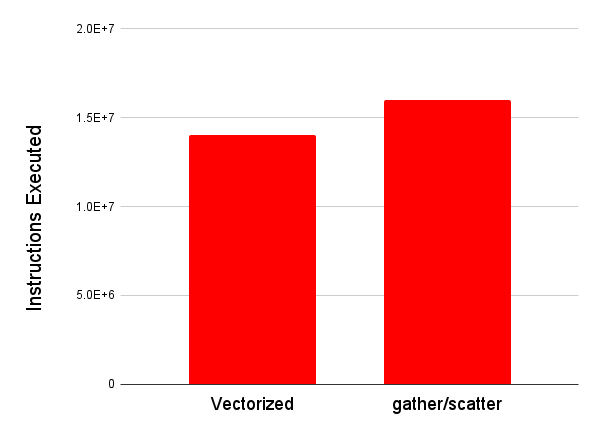
\includegraphics[width=0.99\textwidth]{Figures/gather_scatter_instructions.png}}
\end{minipage}\hfill
\begin{minipage}{.45\textwidth}
\subfloat[Number of Program Cycles]{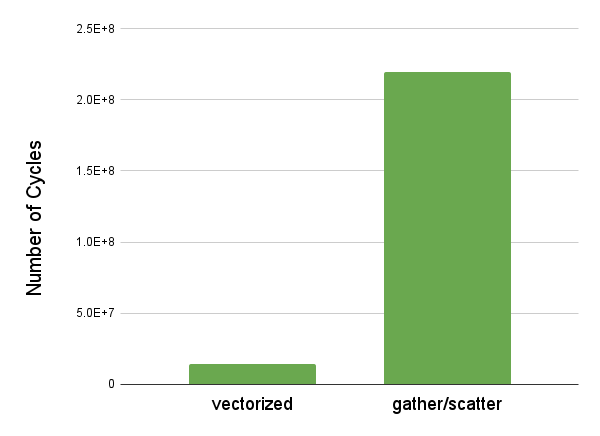
\includegraphics[width=0.99\textwidth]{Figures/gather_scatter_cycles.png}}\hfill
\end{minipage}
\noindent\begin{minipage}{.45\textwidth}
\subfloat[Cycles stalled due to memory]{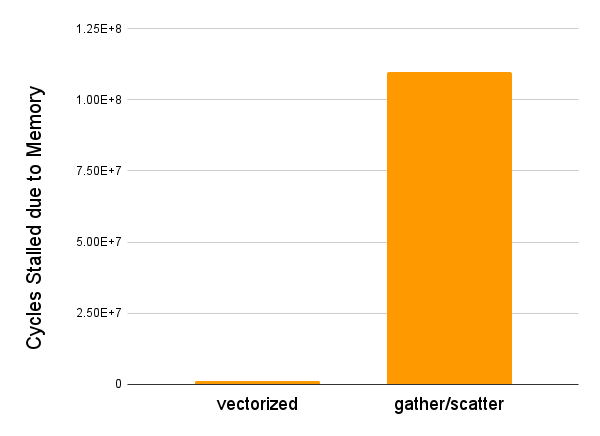
\includegraphics[width=0.99\textwidth]{Figures/gather_scatter_mem_stall.png}}\hfill
\end{minipage}\hfill
\begin{minipage}{.45\textwidth}
\subfloat[Cycles with no instructions executed]{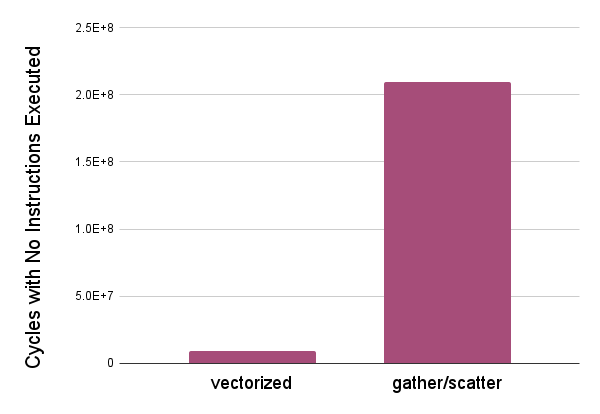
\includegraphics[width=0.99\textwidth]{Figures/gather_scatter_no_instr.png}}
\end{minipage}
 \caption{Performance comparison between predicated instructions and gather/scatter}
\end{figure*}

Listing 5 shows the simple test kernel we use to analyze performance of gather and scatter instructions. It's a simple loop, iterating over an array and copying elements from the input array to the output array only if the corresponding element in the condition array was true. The condition array is designed so that every other element was true, which creates a non-contiguous memory access pattern.

To perform the test, we provide two versions of the code. The first is an if-converted version that uses predicated instructions to perform loads and stores from consecutive memory addresses. 
The second version utilizes gather load and scatter store instructions to load data from the addresses where we knew the corresponding condition is true.


Figure 3 shows a performance comparison between predicated code and the version of code with gather/scatter instructions. 
Figure 3(a) indicates that the difference between the number of instructions that each version executes is not significant. 
However, the execution of the gather/scatter version requires 15x more cycles. 
Results presented in Figures 3(c) and 3(d) shed light on the reason for this significant performance degradation. The number of cycles wasted due to memory stalls increases by almost 10x. 
These results suggest that using gather load and scatter store instructions to eliminate the need to use predicated instructions introduces significant latency overhead.

\subsection{Efficient ALC via Data Permutation}
\label{sec:alc-data-permutation}

ALC as proposed by Wyatt \etal can not eliminate the use of gather/scatter instructions since after permutation, we will have a vector of indices for which we should execute a block and For any Load or store instruction that exists in that block, we need to load/store corresponding indices. As a result, gather/scatter instructions are inevitable.

In this section, we propose our approach to solve this problem. We modify the ALC algorithm so that there will be no need to use gather instructions. To do this, we first detect all load instructions that exits in the blocks that are going to be executed for permuted index vector (for our motivating example, it would be then and else blocks). Then, in the beginning of each loop iterations, for \emph{all detected arrays,} we load \emph{all elements} of that iteration. This will give us \emph{data vectors} that each include elements of an array, that some are going to be used in then block and some in else block. Having these data vectors, we modify the permutation algorithm to permute data vectors \emph{as well as} index vectors.

Figure 3 shows the approach. As explained, initially, we do a vector load for all arrays to load indices of the arrays that corresponds to the current index vector. Since it's a normal vector load and there is no predication, it will load from consecutive memory addresses and it will be fast. Then we do the permutation for both index vector and these data arrays. The rest of the algorithm will be the same as before. After checking the uniform vector, we execute the corresponding block. During executing the block, when we face with a load instruction, we ignore that and whenever the result of that load instruction is used as an operand to an instruction, we will use a permuted data vector.

Data Permutation eliminates all gather instructions at the cost of extra vector loads and executing more instructions for permutation. While these overheads might seem too expensive, our evaluations show that the benefit they bring, covers their overhead. Moreover, it's important to note that although permutation involves executing a significant number of instructions, they are all vector manipulation instructions which only move data between vector, so they are very fast. Our measurements show that, in most cases, permutation takes less than 5\% of loop execution time, suggesting that they will not introduce a significant overhead.  

\begin{figure*}[h]
  \centering
  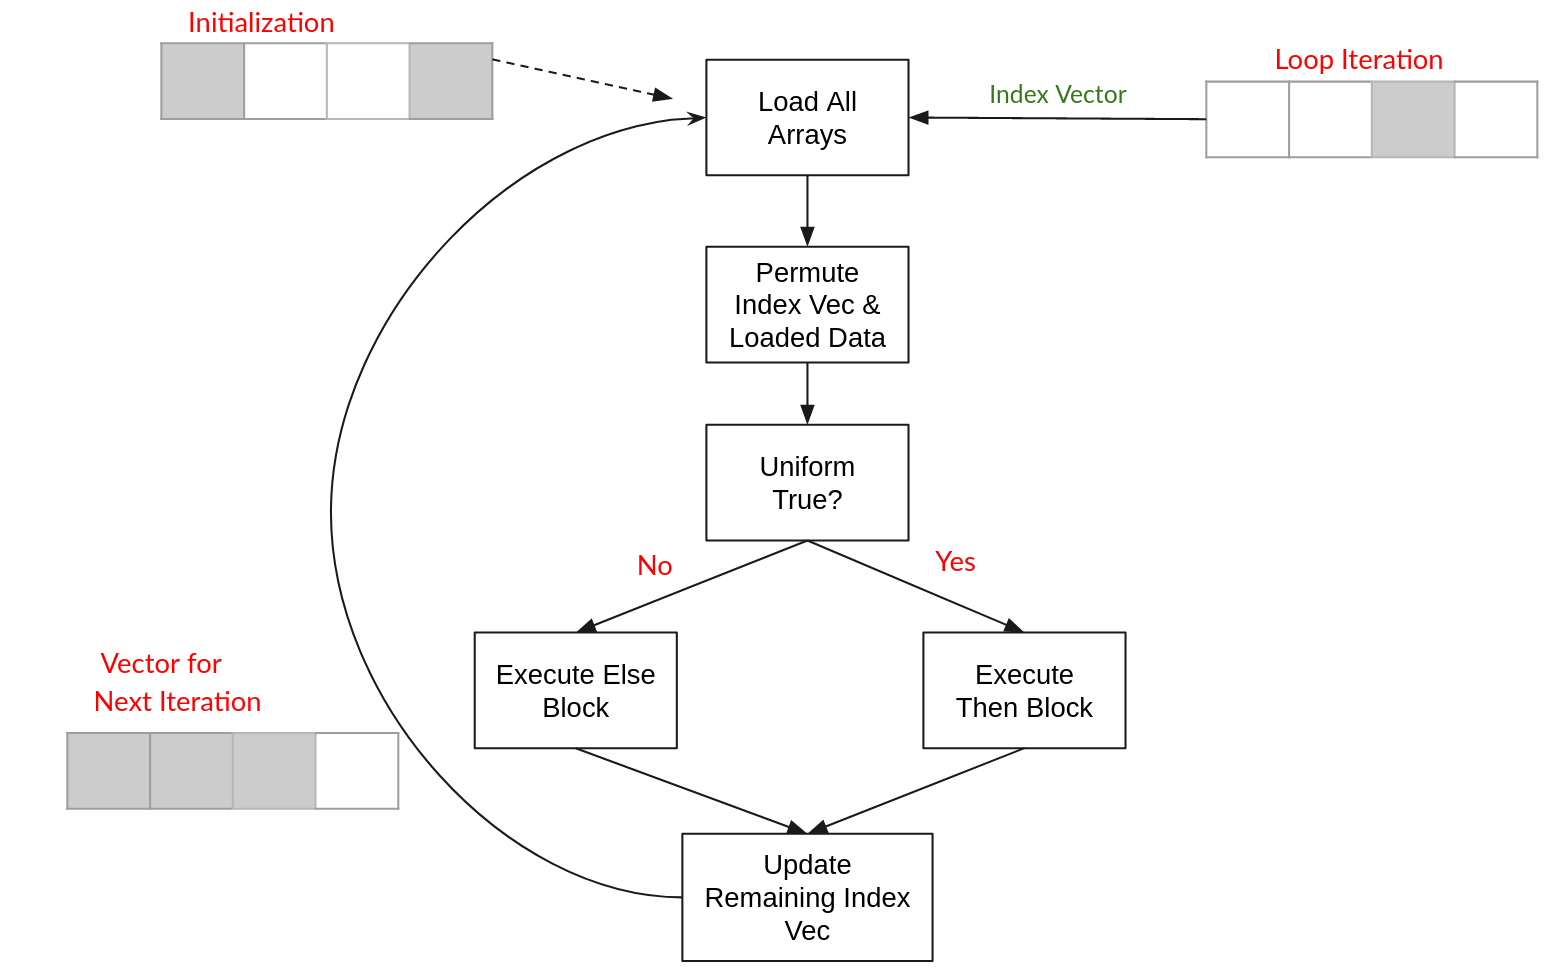
\includegraphics[width=\textwidth]{Figures/data_permute_alg.png}
  \caption{Data Permutation Algorithm}
\end{figure*}

\subsection{Single If Statement}
The algorithm proposed for data permutation is only applicable on the loops that contain a single if-then-else statement. In this section, we explain how we can modify ALC to get performance improvements when applied to the loops containing a single if statement.In figure 1 we demonstrated how vector lanes are wasted due to predication when if-conversion is applied on if-then-else statement, however in the case of single if, it will be different. In such a case, we only loose vector lanes for the false predicates and because there is no else block, we do not execute any extra instruction. This suggests that, if-conversion is already doing good in these cases however, when it comes to an input where majority of the iterations the condition of the loop is false, if-converted code will end-up wasting vector lanes significantly.

With this in mind, we modified the ALC algorithm to utilize both permutation and if-conversion, as illustrated in figure 4. In each iteration, there will be two vector of indices as before. We check to see if enough active lanes exists in \emph{both} index vector. If so, it means that there won't be much vector lanes wasted by predication, so we execute if-converted code. On the other hand, if  there are a few active lanes, the program takes the ALC path where it first does permutation and only if a uniform vector is formed, it executes then block.

The main decision here is, when to execute if-conversion path and when ALC. For this, we define enough active lanes of two vectors to be as follow:

 \begin{math} Enough\_Active\_Lanes = \\
    cntp(FirstVector) + cntp(SecondVector) > VLENGH 
 \end{math}

 where \emph{cntp} is a vector manipulation function that counts the number of true predicates in a given vector and \emph{VLENGTH} is the size of the vector. 
 
 Using this equation For decision of applying ALC in figure 4, we are also able to reduce permutation overhead. In the original permutation algorithm, we had 4 outputs: 2 index vectors and their corresponding predicate vectors. In this case, however, we only do permutation when we are sure that the total number of active lanes in both vectors are smaller than or equal to the size of the vector as a result, the second index vector resulting from permutation will always be uniform false and because there are no else blocks, we can safely ignore that resulting uniform false vector. 

 This modification in permutation algorithm will reduce it's overhead by around 50\%. This becomes more important when we apply data permutation together with ALC on this case.

\begin{figure*}[h]
  \centering
  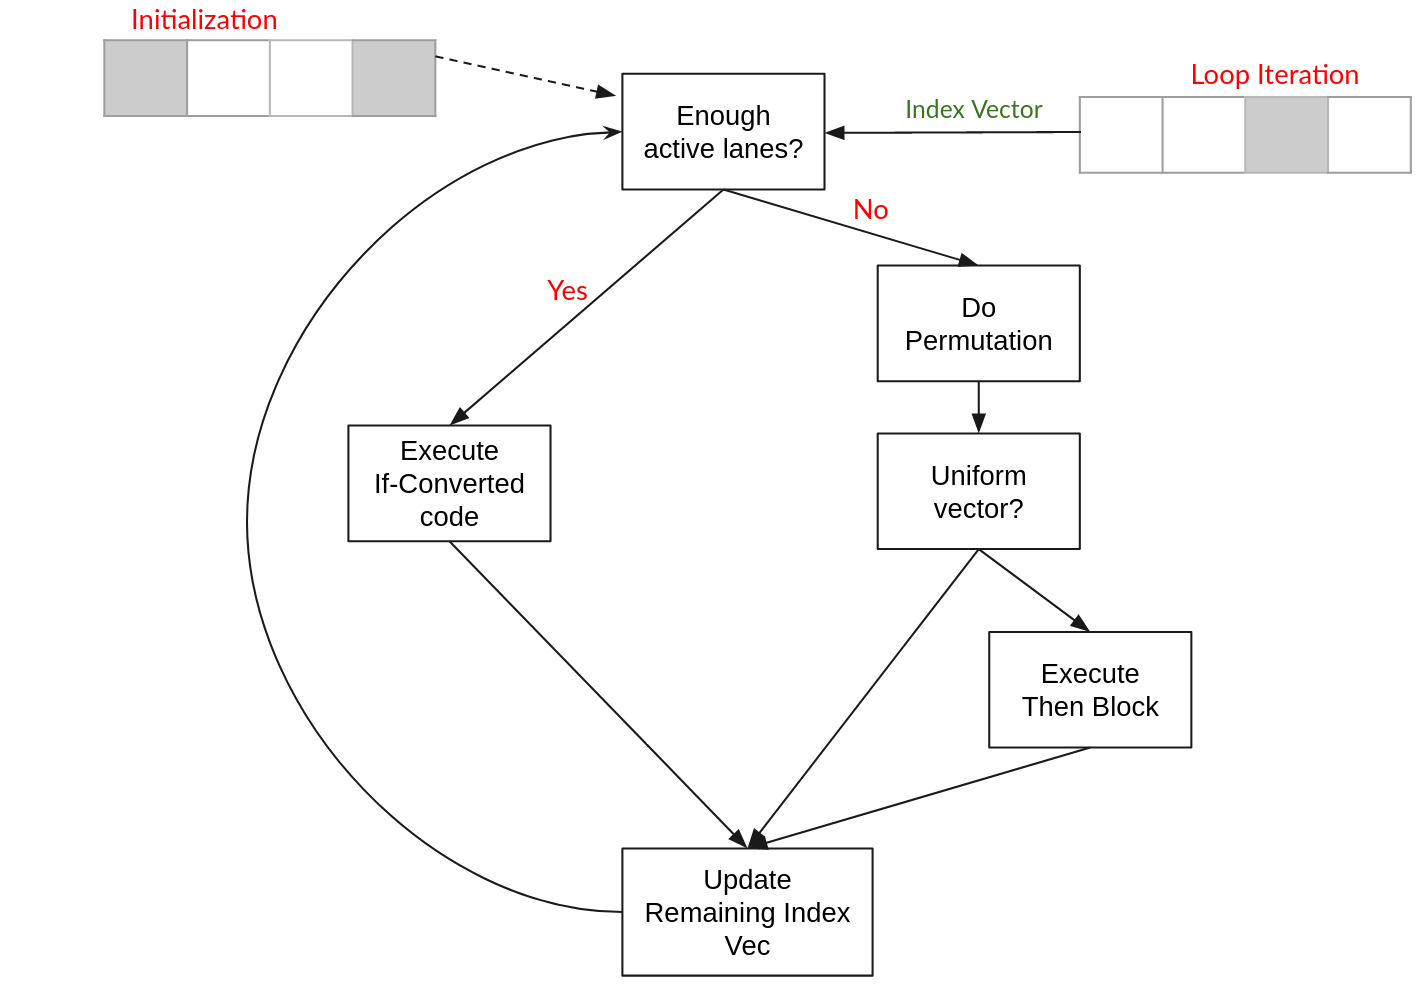
\includegraphics[width=0.8\textwidth, height=10cm]{Figures/ALC_single_if.png}
  \caption{ALC Single if statement Algorithm}
\end{figure*}

% ######  ATTENTION #############
% The content above was left as a reference and is not going to be used for the paper.
% ######  ATTENTION #############
\fi

